\chapter[Gerenciamento do Produto]{Gerenciamento do Produto}

A Engenharia de Produto é responsável por desenvolver o produto e mantê-lo operando. Com a visão de negócios trazida pelo gestor de produto, baseado no entendimento da necessidade ou do problema do cliente, somada ao desenho da solução feito pela equipe com capacidade técnica adequada, a engenharia de produto “constrói” o produto desejado. Para construir o produto ela deve não só fazer a programação, como também definir a arquitetura técnica do produto, ou seja, qual é a arquitetura de hardware do produto, qual a linguagem de programação mais adequada, qual o tratemento dos dados mais apropriado e como garantir os requisitos funcionais e não funcionais do produto. Além disto, o gestor do projeto deve controlar os custos e aquisições de materiais para a construção do produto. 
 
Pelo fato de o gestor de produto ser responsável por definir o produto a ser feito, pode dar a impressão que a engenharia de produtos está subordinada à gestão de produtos, mas essa visão é incorreta e, se as áreas se comportarem dessa forma, a chance de fracasso do produto aumenta, pois quem se sente subordinado tem menos comprometimento com o resultado. A engenharia de produtos e a gestão de produtos são pares, não há relação de subordinação entre nenhuma destas partes. Elas devem funcionar como parceiras, como sócias, cada uma com a sua especialidade e com a sua responsabilidade, colaborando para produzir o melhor resultado possível.

Com isso, dentro do desenvolvimento do Posicionador de Lente, é essencial a integração dos graduandos em Engenharia de Software, que possuem uma capacidade e conhecimento em gestão de projetos e de produtos, de forma que possuem um pensamento sistêmico sobre o produto a ser desenvolvido. Os graduandos das demais áreas, com seus conhecimentos técnico diversificados, agregam esforços para alcançar as características desejadas do Posicionador de Lente. Assim, é importante o papel do gestor do produto para acompanhar, controlar e informar a visão de todo o sistema enquanto a parte técnica está focada em partes mais específicas do produto.

Na figura \ref{gestaoproduto} está ilustrado o diagrama base da gestão do produto dentro do contexto da disciplina Projeto Integrador 2. A engenharia de produtos é aquela que traz a tecnologia disponível. Inovar não é simplesmente conhecer a tecnologia mais recente. É preciso conhecer isto e também todas as tecnologias disponíveis e saber como utilizá-las. Esse é o papel da engenharia de produtos: aplicar tecnologias para resolver um problema ou atender a uma necessidade de um grupo. A gestão do produto lida com os três pilares: conhecer a tecnologia disponível e coordenar o desenvolvimento ou "inovação" de um produto, atender as necessidades dos possíveis usuários e atingir os objetivos definidos dentro da disciplina Projeto Integrador 2.

\begin{figure}[H]
		\centering
			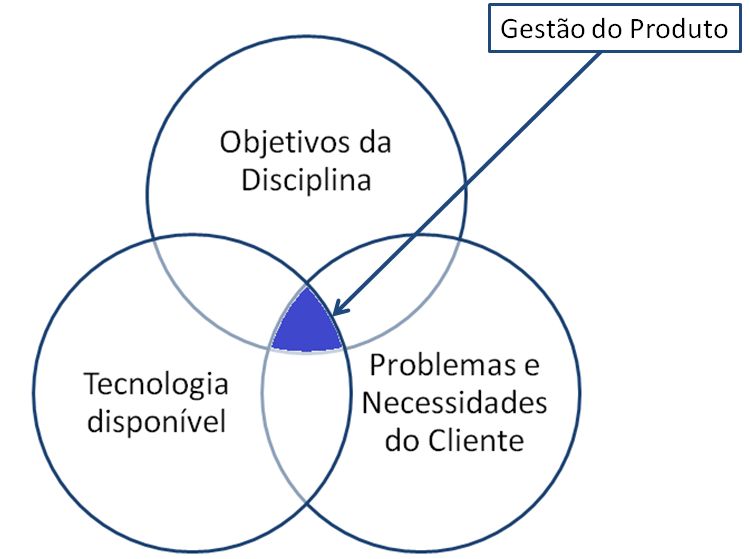
\includegraphics[scale=0.6]{figuras/gestaoproduto.png}
		\caption{Diagrama da Gestão do Produto}
		\label{gestaoproduto}
\end{figure}

Com isso, uma engenheira de software, baseada no aprendizado adquirido dentro do curso, definiu alguns procedimentos que serão executados por ela dentro do papel de gestora do produto a fim de facilitar o dia a dia junto aos engenheiros do produto (engenheiros automotivos, de energia e de eletrônica). São eles:

\begin{itemize}
\item Evitar palpitar sobre a solução técnica sem uma pesquisa ou conhecimento anterior sobre o tema. Um gestor de produto deve ter algum conhecimento técnico sobre seu produto, mas essa não é sua área de especialidade. Os especialistas estão na equipe de engenharia de produto. Por isso, é preciso acompanhar de perto as soluções técnicas proposta e propor outra solução quando possuir o conhecimento adequado sobre o assunto.
\item Deixar todos os membros da equipe informados das conversas com clientes, coordenadores ou idealizadores do produto. O gestor de produto deve conversar sempre com os clientes do produto para entender como ele resolverá o problema ou atenderá às necessidades desse cliente ou como pode melhorar o produto que está sendo desenvolvido. Manter todos informados sobre o que foi conversado e o impacto do produto deixa os engenheiros do produto mais engajados na missão de fazer um produto melhor.
\item Tirar o excesso. O gestor do produto deve buscar sempre o produto mínimo ou a funcionalidade mínima, ou seja, procurar orientar o desenvolvimento do mínimo produto possível para atingir o seu objetivo do negócio. Assim, evitando que tempo e custo sejam desperdiçados com funcionalidades que o cliente não deseja. 
\item Estar presente. É fundamental estar junto com a equipe de engenharia de produto. Durante o desenvolvimento do produto inevitavelmente surgirão dúvidas e sem alguém para organizar e colher opiniões cada um dos subgrupos vai desenvolver como eles acham que deve ser, o que pode ser diferente do que havia sido planejado ou do que o cliente deseja.
\item Dar \textit{feedback} à equipe sobre o produto. O gestor de produto deve saber como o projeto está caminhando e como o que está sendo desenvolvido está ajudando a atingir os objetivos da disciplina. Ao conversar periodicamente sobre isso com a equipe, mostra-se um contexto e um propósito para eles. 
\item Controlar os custos do projeto. Reunir e arrecadar dos membros da equipe o que é necessário para aquisição de materiais para desenvolvimento do produto.
\item Integrar, desenvolver e revisar o relatório do produto.
\end{itemize}
